
\chapter{Stellar spots cause measurable variations in atmospheric metallicity}
\label{chap:stellar_spots}

\textbf{Preamble}

This chapter was originally published as:
\begin{quote}
	\citet{tanner_ss}
\end{quote}
and is presented in the form that it was published \update{in accordance with Monash University's thesis by submission guidelines.}

\newpage

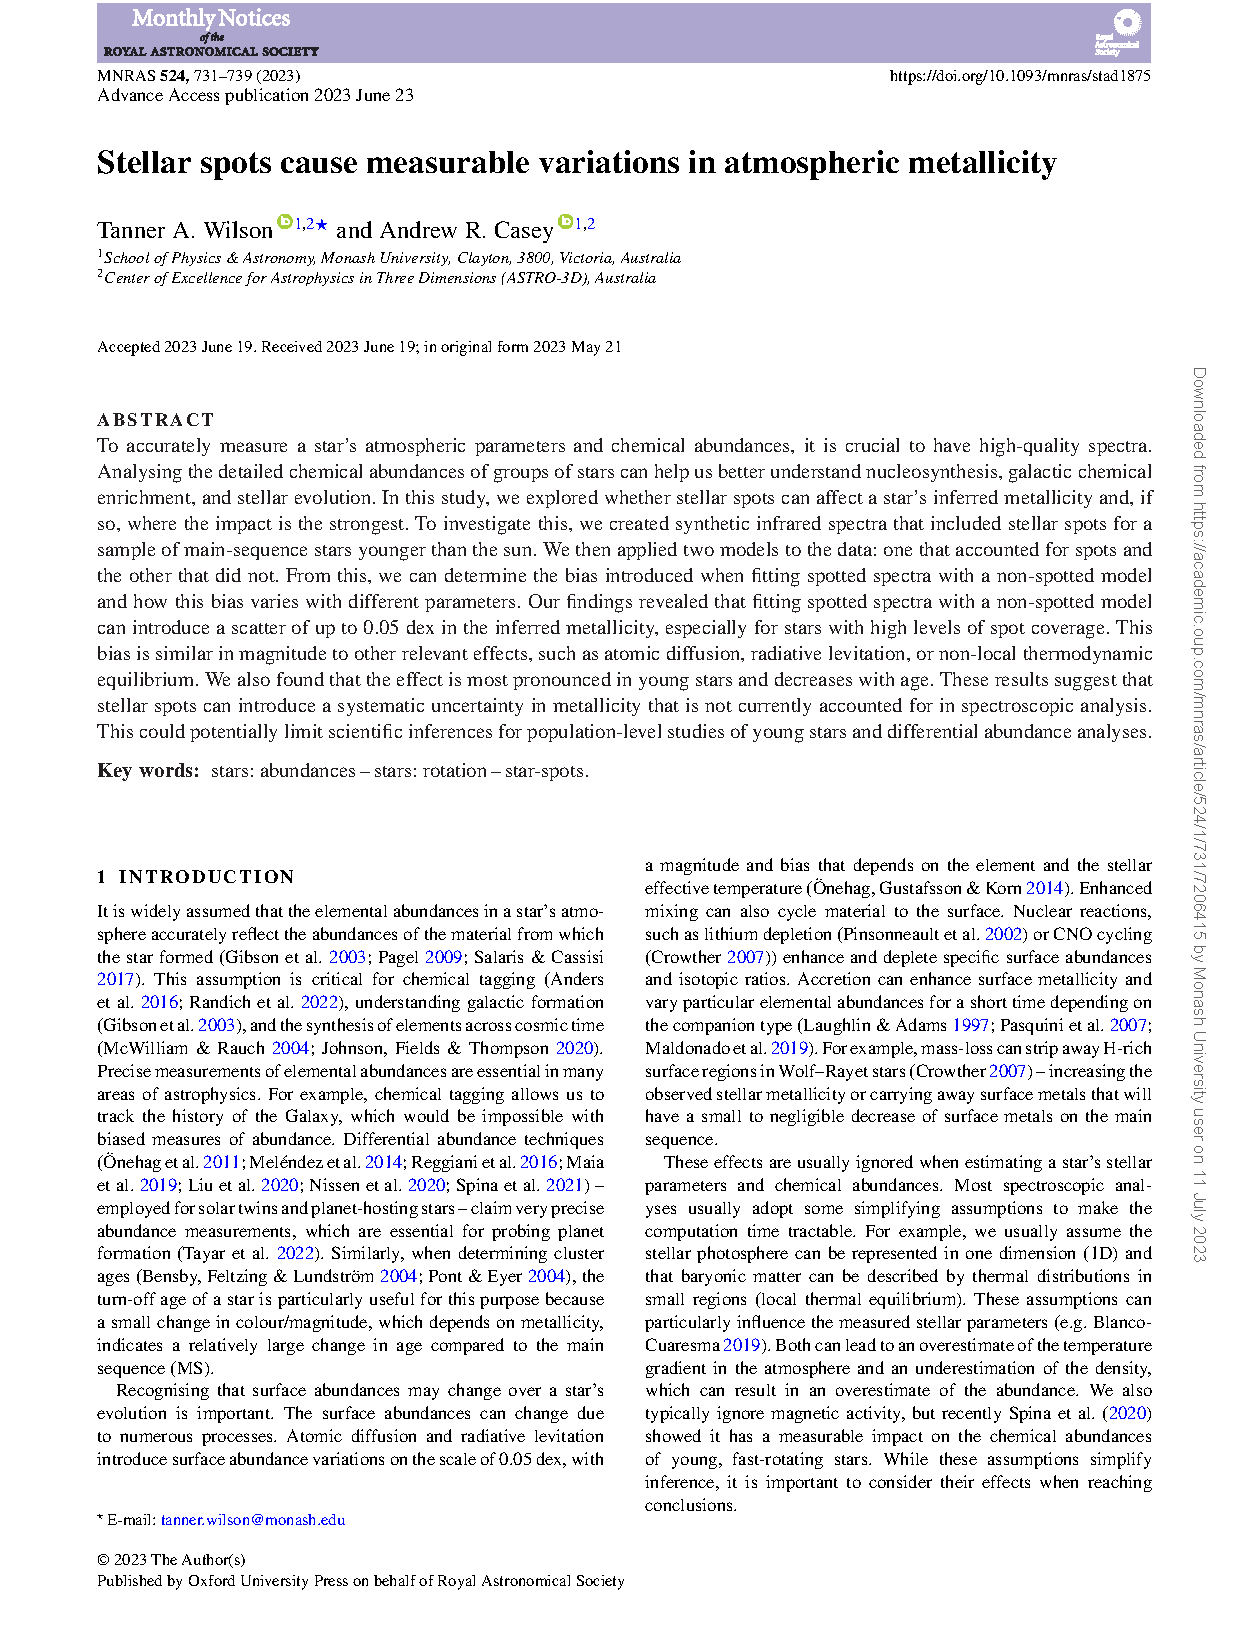
\includepdf[pages =1, pagecommand={}, scale=0.9,offset=65 -50]{Chapters/stad1875-TW-SS.pdf}

\includepdf[pages =2, pagecommand={
\begin{figure}
    \resizebox{!}{0cm}{\begin{minipage}{\textwidth}
    \includegraphics[width=0.5\textwidth]{Figures/ss_chapter_figures/injected_hr.png}
    \caption[HR diagram of the 1500 sets of stellar parameters drawn from physically motivated distributions of mass, metallicity and age coloured by \feh.]{}
    \label{fig:HR}
        \end{minipage}}
\end{figure}
}, scale=0.9,offset=65 -50]{Chapters/stad1875-TW-SS.pdf}

\includepdf[pages =3, pagecommand={
\begin{figure*}
    \resizebox{!}{0cm}{\begin{minipage}{\textwidth}
    \includegraphics[width = \textwidth]{Figures/ss_chapter_figures/recov_tests_spot.png}
    \caption[Recovered traditional stellar parameters (\teff, \logg, \feh \ and \vsini) from fitting synthetic spotted spectra with a spotted model of the stellar atmosphere against the corresponding injected parameters.]{}
    \label{fig:recov_test}
            \end{minipage}}
\end{figure*}}, scale=0.9,offset=65 -50]{Chapters/stad1875-TW-SS.pdf}

\includepdf[pages =4, pagecommand={
\begin{figure}
    \resizebox{!}{0cm}{\begin{minipage}{\textwidth}
    \includegraphics[width=0.5\textwidth]{Figures/ss_chapter_figures/recov_spot_param.png}
    \caption[Recovered spot parameters from the synthetic spotted spectra fitted with a spotted model of the stellar spectra against the injected parameters of the synthetic spectra.]{}
    \label{fig:recov_spot_params}
                \end{minipage}}
\end{figure}}, scale=0.9,offset=65 -50]{Chapters/stad1875-TW-SS.pdf}

\includepdf[pages =5, pagecommand={
\begin{figure*}
    \resizebox{!}{0cm}{\begin{minipage}{\textwidth}
    \includegraphics[width=\textwidth]{Figures/ss_chapter_figures/recov_tests_full.png}
    \caption[The difference between the recovered traditional stellar spectra parameters (\teff, \ \logg, \ \feh \ and \vsini) from the synthetic spotted spectra fitted with both a spotted and non-spotted model of the stellar spectra against the injected parameters of the synthetic spectra]{}
    \label{fig:recov_dif}
                    \end{minipage}}
\end{figure*}}, scale=0.9,offset=65 -50]{Chapters/stad1875-TW-SS.pdf}

\includepdf[pages =6, pagecommand={\begin{figure*}
    \resizebox{!}{0cm}{\begin{minipage}{\textwidth}
    \includegraphics[width=\textwidth]{Figures/ss_chapter_figures/full_results_teff.png}
    \caption[Bias introduced to \teff\ (blue) when fitting spotted spectra with a non-spotted model against injected parameters of synthetic spectra.]{}
    \label{fig:res_teff}
    \end{minipage}}
\end{figure*}}, scale=0.9,offset=65 -50]{Chapters/stad1875-TW-SS.pdf}

\includepdf[pages =7, pagecommand={\begin{figure*}
    \resizebox{!}{0cm}{\begin{minipage}{\textwidth}
    \includegraphics[width=\textwidth]{Figures/ss_chapter_figures/full_results.png}
    \caption[Bias introduced to \logg  \ (orange), \feh \ (green) and $\log$ \vsini\ (red) when fitting spotted spectra with a non-spotted model against injected parameters of synthetic spectra.]{}
    \label{fig:res_full}
        \end{minipage}}
\end{figure*}}, scale=0.9,offset=65 -50]{Chapters/stad1875-TW-SS.pdf}

\includepdf[pages =8, pagecommand={\begin{figure}
    \resizebox{!}{0cm}{\begin{minipage}{\textwidth}
    \includegraphics[width=0.5\textwidth]{Figures/ss_chapter_figures/med_age.png}
    \caption[Bias introduced to \feh \ when fitting spotted spectra with a non-spotted model against the age of the model used to generate synthetic spectra.]{}
    \label{fig:age_mad}
            \end{minipage}}
\end{figure}}, scale=0.9,offset=65 -50]{Chapters/stad1875-TW-SS.pdf}
\includepdf[pages =9, pagecommand={}, scale=0.9,offset=65 -50]{Chapters/stad1875-TW-SS.pdf}

